% !TeX spellcheck = en_US
\documentclass[12pt,a4paper]{article}
\usepackage[utf8]{inputenc}
\usepackage[german]{babel}
\usepackage[T1]{fontenc}
\usepackage{amsmath}
\usepackage{amsfonts}
\usepackage{amssymb}
\usepackage{graphicx}
\usepackage[left=2.5cm,right=2.5cm,top=2cm,bottom=2cm]{geometry}
\usepackage{float}

\usepackage{subcaption}
\usepackage{siunitx}
\usepackage{verbatim} 


\author{Gruppe A2 \\ Julián Häck, Maria Spethmann}
\title{Protokoll Optik 1 \\ Physikalisches Grundpraktikum 2}


\begin{document}
	\maketitle
	\thispagestyle{empty} % Keine Seitenzahl auf der Titelseite
	\newpage
	\pagestyle{headings} % Seitenzahlen oben, Section und Subsection in Kopfzeile
	\tableofcontents
	\newpage


\section{Physikalische Grundlagen}

Ziel dieses Versuchs ist es, die Dispersionskurve $n(\lambda)$ eines Prismas unbekannten Materials zu bestimmen. Dazu wird die Ablenkung der Spektrallinien einer Quecksilber-Cadium-Lampe mithilfe eines Prismenspektrometers gemessen. Nachdem die Dispersionskurve bestimmt wurde, wird das Spektrum einer Zinklampe vermessen und die berechneten Wellenlängen mit Literaturwerten verglichen. Schließlich wird das Auflösungsvermögen des Prismas anhand der gelben Hg-Doppellinie ermittelt.\\\\
\textbf{Dispersion}\\
Der Brechungsindex $n$ ist wellenlängenabhängig, weil die Anregung der Elektronen in einem Medium durch das Verhältnis zwischen Eigenfrequenz der Elektronen und Frequenz der elektromagnetischen Welle bestimmt wird. Im Bereich des sichtbaren Lichtes lässt sich die Dispersionskurve $n(\lambda)$ durch die Cauchy-Gleichung annähern
\begin{equation}\label{eq:Cauchy-Gleichung}
n(\lambda)=a+\frac{b}{\lambda^2}+\frac{c}{\lambda^4},
\end{equation}
wobei $a$, $b$ und $c$ materialabhängige Konstanten sind.\\\\
\textbf{Prisma}
\begin{figure}[H]
	\centering
	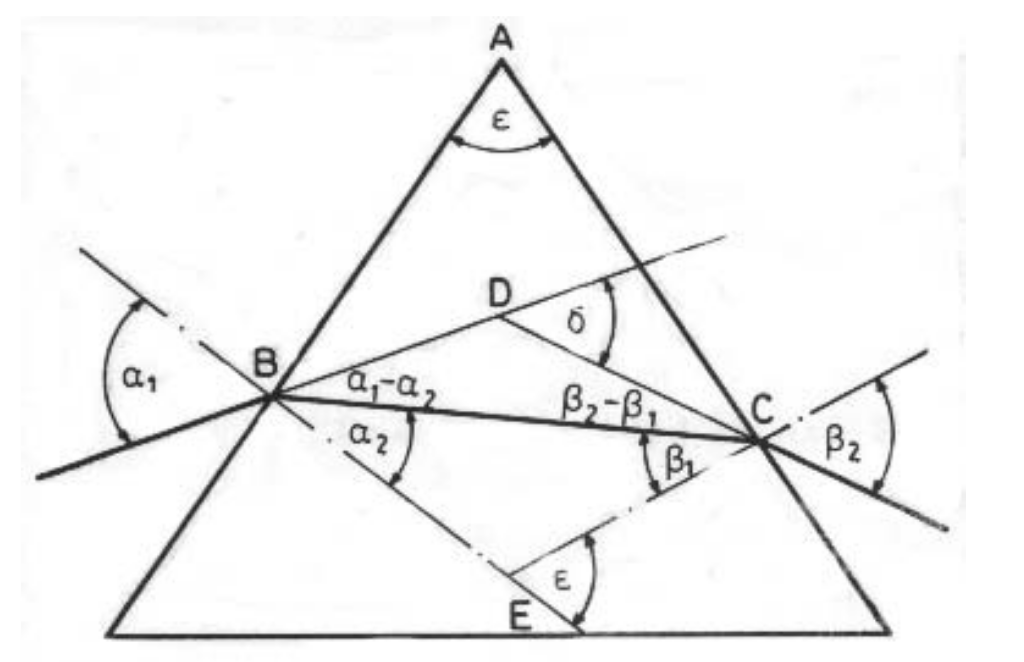
\includegraphics[width=0.8\textwidth]{Bilder/Prisma_Strahlengang.png}
	\caption{Strahlengang durch das Prisma}
	\label{Prisma_Strahlengang}
\end{figure}
 Das Snelliussche Brechungsgesetz bezieht Einfallswinkel $\alpha_1$, Brechungswinkel $\alpha_2$ und die Brechungsindexe der Medien aufeinander:
\begin{equation}
n_1 \cdot sin(\alpha) = n_2 \cdot sin(\beta)
\end{equation}
Mithilfe dieses Gesetzes und geometrischen Zusammenhängen kann der Strahlengang durch ein Prisma berechnet werden. Letztendlich hängt der Ablenkwinkel $\delta$ des Lichtstrahls auf folgende Weise von dem Einfallswinkel $\alpha_1$, dem brechenden Winkel $\epsilon$ und dem Brechungsindex $n$ des Prismas ab:
\begin{equation}
\delta=\alpha_1-\epsilon+\arcsin{\left(\sqrt{n^2-\sin^2{\alpha_1}}\sin{\epsilon}-\sin{\alpha_1}\cos{\epsilon}\right)}.
\end{equation}
Der Ablenkwinkel $\delta$ wird minimal für den symmetrischen Strahlendurchgang, bei dem der Austrittwinkel $\beta_2$ gleich dem Einfallswinkel $\alpha_1$ ist. In diesem Fall gilt folgender Zusammenhang zwischen Minimalablenkung und Brechungsindex:
\begin{equation}\label{eq:n_aus_delmin}
n=\frac{\sin((\delta_{min}+\epsilon)/2)}{\sin(\epsilon/2)}.
\end{equation}
In diesem Versuch wird die Minimalablenkung $\delta_{min}$ bekannter Spektrallinien des Cadiums- und Quecksilberspektrums gemessen und daraus der Brechungsindex berechnet. Nun können die Koeffizienten $a$, $b$ und $c$ aus  Gl.~\eqref{eq:Cauchy-Gleichung} mit einer Ausgleichsrechnung bestimmt werden.\\\\
\textbf{Auflösungsvermögen}\\
Eine charakterisierende Größe eines Prismas ist sein Auflösungsvermögen $A$. Es wird definiert als 
\begin{equation}
A=\frac{\lambda}{\Delta\lambda}
\end{equation}
und beschreibt die benötigte Wellenlängendifferenz $\Delta\lambda$, um zwei Spektrallinien mit Wellenlängen $\lambda$ und $\lambda+\Delta\lambda$ noch mit dem Prisma trennen zu können. Bei symmetrischem Strahlengang und voller Ausleuchtung lässt sich das Auflösungsvermögen des Prismas berechnen durch
\begin{equation}
A=S\frac{dn}{d\lambda}
\end{equation}
mit Prismenbasis $S$.
\section{Versuchsaufbau und -durchführung}
Ein Prismenspektrometer besteht aus einer Lichtquelle, einem festen Kollimator, einem Prisma auf einer Drehscheibe und einem schwenkbaren Fernrohr, dessen Winkeleinstellung bezüglich eines festen Teilkreises auf eine Bogenminute genau abgelesen werden kann. Das Licht der Spektrallampe fällt über einen die Intensität regelnden Spalt in den Kollimator und wird an der Kollimatorlinse in ein ebenes Lichtbündel umgewandelt. Das Lichtbündel fällt auf das Prisma und wird in Abhängigkeit von Einfallswinkel und Wellenlänge abgelenkt. Nun kann das abgelenkte Bild des Spaltes durch das Fernrohr, welches aus einer Objektiv- und einer Okularlinse besteht, vergrößert betrachtet werden. Der Strahlengang durch das Spektrometer wird in Abb.~\ref{Spektrometer_Aufbau} dargestellt. Abb.~\ref{Aufbau_Foto} zeigt eine Übersicht über den Versuchsaufbau.\\
Man betrachtet nun durch das Fernrohr eine Spektrallinie und variiert durch Drehung der Prismadrehscheibe den Einfallswinkel. Ein symmetrischer Strahlendurchgang mit Minimalablenkung ist dann erreicht, wenn sich bei gleichsinniger Drehung des Prismas die Laufrichtung des Spaltbildes durch das Fernrohr umkehrt. Man schwenkt den Fernrohrarm so, dass sich das Fadenkreuz des Fernrohrs dann auf dem Spalt befindet, wenn die Minimalablenkung erreicht ist, und notiert den Winkel der Fernrohrposition $\psi_1$. Anschließend dreht man das Prisma um, sodass das Licht auf die andere Seite gebrochen wird, wiederholt den beschriebenen Prozess zum Finden des symmetrischen Strahldurchgangs und misst den zweiten Winkel $\psi_2$, der zur gleichen Spektrallinie gehört. Die Minimalauslenkung $\delta_{min}$ lässt sich nun wie folgt berechnen:
\begin{equation}\label{eq:delmin_aus_psi}
\delta_{min}=\frac{\psi_1-\psi_2}{2}
\end{equation}
\subsection{Bestimmung der Dispersionskurve}
Zunächst verwenden wir eine CdHg-Lampe und messen für die 8 Wellenlängen aus Tabelle \ref{table:Winkel_Rohdaten} jeweils drei Mal die linksseitigen und rechtsseitigen Umkehrwinkel $\psi_1$ und $\psi_2$. Die Werte werden gemittelt und der Brechungsindex in Abhöngigkeit der 8 Wellemlängen mithilfe von Gl.~\eqref{eq:delmin_aus_psi} und Gl.~\eqref{eq:n_aus_delmin} berechnet. Um den Fehler der Messgenauigkeit abschätzen zu können, wird $\psi_1$ der roten Spektrallinie von Quecksilber 10 Mal bestimmt. Die Unsicherheit auf dieses $\psi_1$ wird auf die anderen Messungen übertragen. Die Annahme, dass die Unsicherheiten auf die $\psi$ gleich groß sind, ist möglich, weil alle Messungen von einem Experimentator durchgeführt wurden. Das benutzte Prisma hat laut Hersteller einen brechenden Winkel von $\ang{60}$. \\\\
\subsection{Vermessen eines unbekannt Spektrums}
Nachdem die Dispersionskurve bestimmt wurde, wird das Spektrum einer Zinklampe vermessen. Wie im vorherigen Teil werden dafür jeweils drei links- und rechtsseitige Umkehrwinkel $\psi_1$ und $\psi_2$ gemessen zu vier verschiedenen Spektrallinien. Mithilfe der Dispersionskurve kann nun die Wellenlänge dieser Spektrallinien berechnet werden und mit den Literaturwerten verglichen werden.\\\\
\subsection{Auflösungsvermögen}
Schließlich wird das Auflösungsvermögen des Prismas bei unterschiedlicher Ausleuchtung anhand der gelben Hg-Doppellinie bestimmt. Dazu wird eine verschiebbare Schlitzblende verwendet, die an das vordere Ende des Kollimators befestigt wird. Die Spaltbreiten $a$ lassen sich in Schritten von 0.5mm von $a=0.5mm$ bis $a=6mm$ einstellen und bestimmen die Breite des Lichtbündels, das auf das Prisma fällt. Das Auflösungsvermögens des Prismas ist somit bestimmbar durch
\begin{equation}
A=\frac{dn}{d\lambda}2a\frac{\sin{\frac{\epsilon}{2}}}{\cos{\frac{\delta_{min}+\epsilon}{2}}}.
\end{equation}
Die Spaltbreite wird zu kleineren Werten hin variiert und der Wert für $a$ notiert, bei der die Hg-Doppellinie gerade nicht mehr auflösbar erscheint.

\begin{figure}
	\centering
	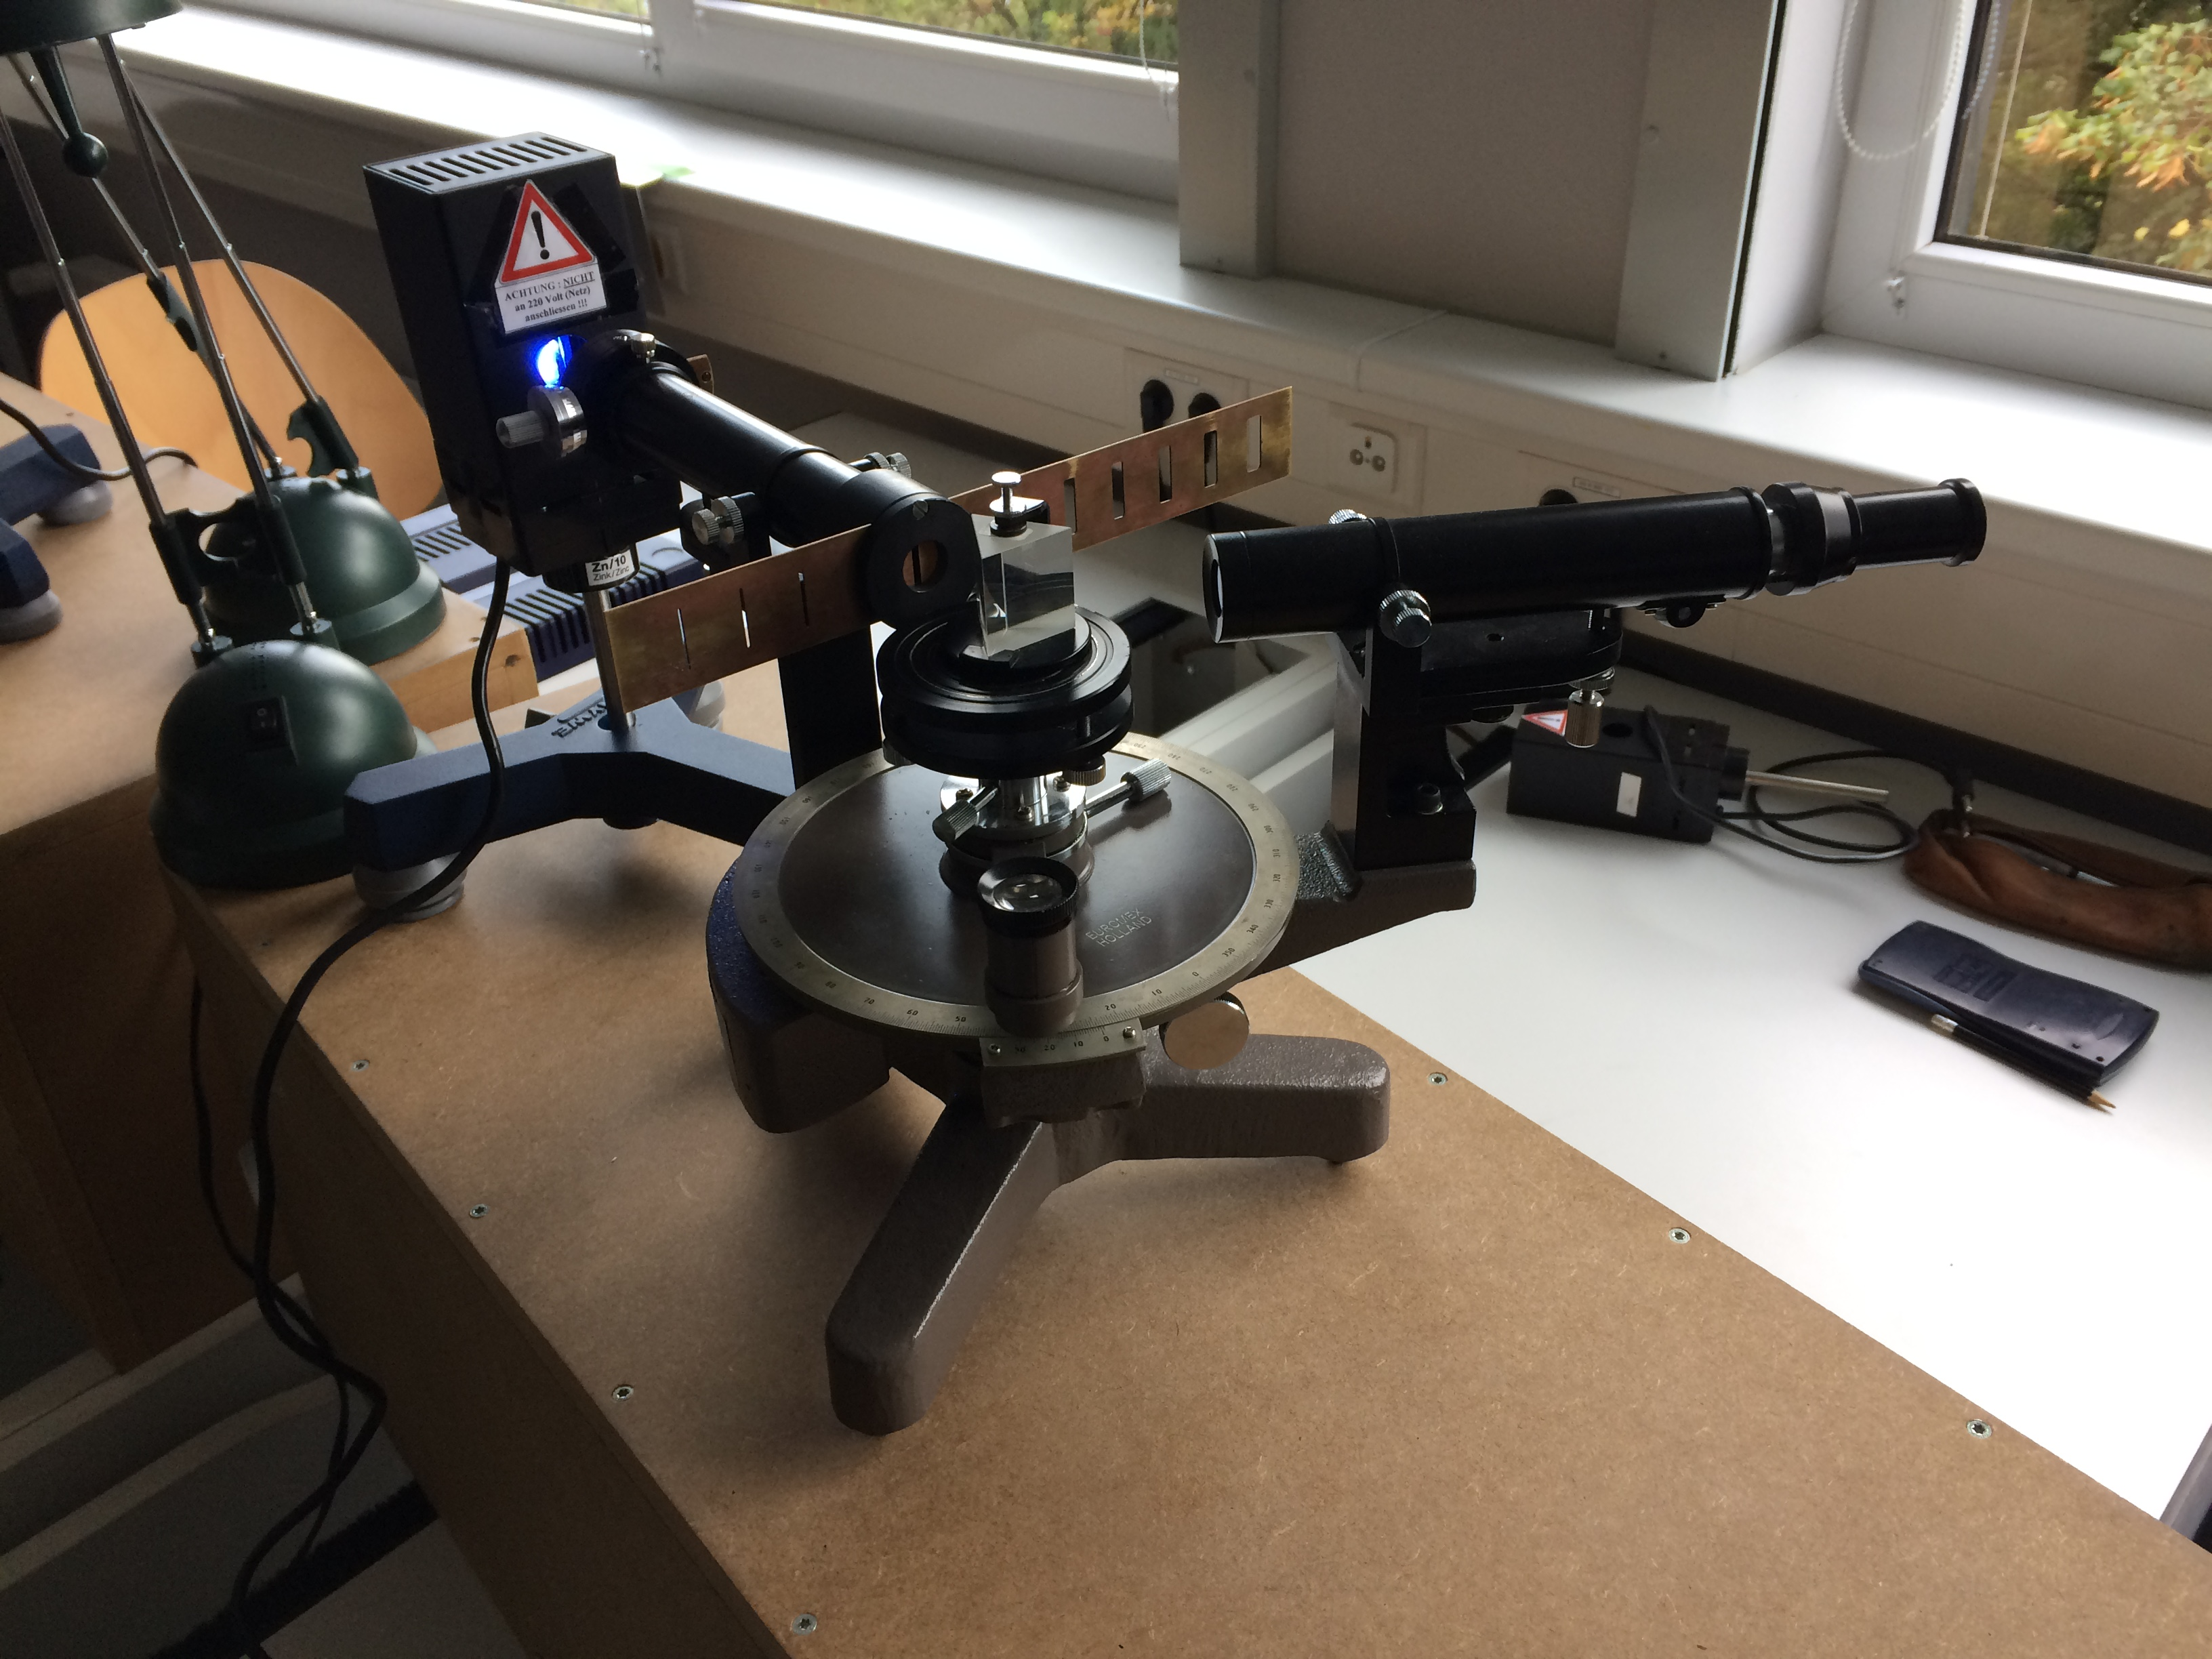
\includegraphics[width=0.9\textwidth]{Bilder/Aufbau_Foto.jpg}
	\caption{Versuchsaufbau}
	\label{Aufbau_Foto}
\end{figure}

\begin{figure}
	\centering
	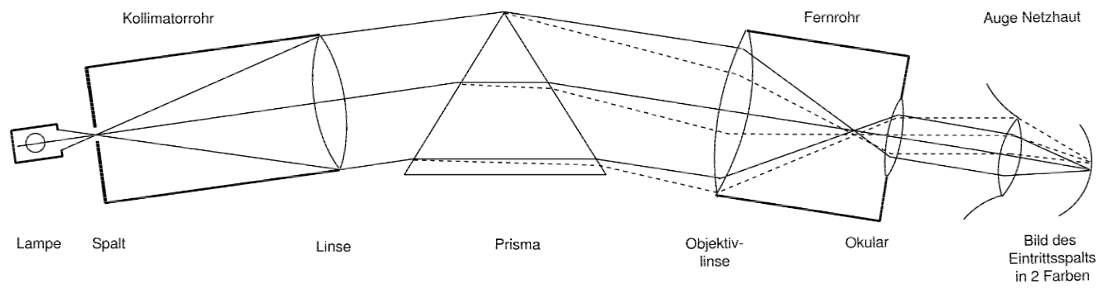
\includegraphics[width=0.9\textwidth]{Bilder/Spektrometer_Aufbau.png}
	\caption{Versuchsaufbau: Strahlengang durch das Spektrometer}
	\label{Spektrometer_Aufbau}
\end{figure}

\section{Auswertung}



\subsection{Bestimmung der Messunsicherheit auf  $\phi_i$}
Die gemessenen Werte für $\psi_{1}$ und $\psi_2$ sind in Tabelle \ref{table:Winkel_Rohdaten} zusammengefasst. Zur Bestimmung der Messunsicherheit auf $\psi$ verwendet wir die 10 linksseitigen Messungen $\psi_1$ der roten Quecksilberlinie. 
Wir berechnet die Standardabweichung der Verteilung durch
\begin{equation}
\sigma_{\psi}=\sqrt{\frac{1}{N-1}\sum^{N}_{i=1}{(\psi-\overline{\psi})^2}}
\end{equation}
mit $N=10$ und nehmen an, dass diese Unsicherheit auch für die anderen Werte von $\psi_1$ und $\psi_2$ gilt. Die Berechnung ergibt
\begin{equation}
\sigma_{\psi}=\ang{0.01372}.
\end{equation}
Die Unsicherheit auf den Mittelwert einer Größe erhält man nun durch
\begin{equation}
\sigma_{\overline{\psi}}=\frac{\sigma_{\psi}}{\sqrt{N}}
\end{equation}
bei N Messungen.  In unserem Fall ergibt sich für drei Messungen $\sigma_{\overline{\psi}}=\ang{0.00792}$. Da der Wert größer ist als die Ableseungenauigkeit von $\sigma_{\psi, Messskala}=\frac{\ang{1}}{60\sqrt{12}}=\ang{0.0048}$ verwenden wir ersteres als Unsicherheit auf $\overline{\psi}$. Bei den 10 Messungen der linksseitigen roten Quecksilberlinie ist dagegen die Unsicherheit, die sich durch die Messskala ergibt, größer, sodass wir dort mit $\sigma_{\overline{\psi}}=\ang{0.0048}$ weiterrechnen.


\subsection{Bestimmung der Dispersionskurve $n(\lambda)$ mit der Cauchy Formel}
Nun berechnen wir aus den gemittelten linksseitigen und rechtsseitigen Umkehrwinkeln die Minimalablenkung $\delta_{min}$ und den Brechungsindex $n$ gemäß Gl.~\eqref{eq:delmin_aus_psi} und Gl.~\eqref{eq:n_aus_delmin}. Die Unsicherheiten auf $\delta_{min}$ und $n$ werden durch Fehlerfortpflanzung ermittelt und sind statistischer Natur.
\begin{align}
\sigma_{\delta_{min}}&=\sqrt{\frac{\sigma_{\overline{\psi_1}}^2+\sigma_{\overline{\psi_2}}^2}{2}}\\
\sigma_n&=\Big|\frac{1}{2\sin{\frac{\epsilon}{2}}}\cos{\left(\frac{\epsilon+\delta_{min}}{2}\right)}\sigma_{\delta_{min}}\Big|
\end{align}
Die systematische Unsicherheit auf $\epsilon$ und $\lambda$ ist sehr klein und wird im Folgenden vernachlässigt. Die Werte für  $\delta_{min}$, $n$ und ihre Fehler werden in Tabelle \ref{table:CdHg_Rechnung} zusammengefasst.\\


\begin{table}
	\centering
	\begin{tabular}{|c|c|c|}
		\hline
		 & Winkel $\psi_{1i}$ in Grad & Winkel $\psi_{2i}$ in Grad\\
		\hline
		Quecksilber&$322.5+\frac{14}{60}$&$204.5+\frac{13}{60}$\\[0.1cm]
		rot&$322.5+\frac{14}{60}$&$204.5+\frac{15}{60}$\\[0.1cm]
		$\lambda=643.85nm$&$322.5+\frac{14}{60}$&$204.5+\frac{15}{60}$\\[0.1cm]
		&$322.5+\frac{14}{60}$&\\[0.1cm]
		&$322.5+\frac{13}{60}$&\\[0.1cm]
		&$322.5+\frac{13}{60}$&\\[0.1cm]
		&$322.5+\frac{12}{60}$&\\[0.1cm]
		&$322.5+\frac{12}{60}$&\\[0.1cm]
		&$322.5+\frac{13}{60}$&\\[0.1cm]
		&$322.5+\frac{14}{60}$&\\[0.1cm]
		\hline
		Quecksilber&$323.5+\frac{3}{60}$&$203.5+\frac{23}{60}$\\[0.1cm]
		gelb&$323.5+\frac{3}{60}$&$203.5+\frac{21}{60}$\\[0.1cm]
		$\lambda=579.07nm$&$323.5+\frac{3}{60}$&$203.5+\frac{23}{60}$\\[0.1cm]
		\hline
		Quecksilber&$324+\frac{6}{60}$&$203+\frac{20}{60}$\\[0.1cm]
		hellgrün&$324+\frac{8}{60}$&$203+\frac{19}{60}$\\[0.1cm]
		$\lambda=546.07nm$&$324+\frac{5}{60}$&$203+\frac{20}{60}$\\[0.1cm]
		\hline
		Cadmium&$324.5+\frac{23}{60}$&$202.5+\frac{0}{60}$\\[0.1cm]
		dunkelgrün&$324.5+\frac{25}{60}$&$202.5+\frac{0}{60}$\\[0.1cm]
		$\lambda=508.58nm$&$324.5+\frac{25}{60}$&$202.5+\frac{1}{60}$\\[0.1cm]
		\hline
		Cadmium&$325.5+\frac{14}{60}$&$201.5+\frac{13}{60}$\\[0.1cm]
		hellblau&$325.5+\frac{14}{60}$&$201.5+\frac{13}{60}$\\[0.1cm]
		$\lambda=479.99nm$&$325.5+\frac{13}{60}$&$201.5+\frac{12}{60}$\\[0.1cm]
		\hline
		Cadmium&$326+\frac{6}{60}$&$201+\frac{18}{60}$\\[0.1cm]
		dunkelblau&$326+\frac{6}{60}$&$201+\frac{18}{60}$\\[0.1cm]
		$\lambda=467.81nm$&$326+\frac{7}{60}$&$201+\frac{17}{60}$\\[0.1cm]
		\hline
		Quecksilber&$327+\frac{25}{60}$&$200+\frac{1}{60}$\\[0.1cm]
		violett&$327+\frac{23}{60}$&$200+\frac{0}{60}$\\[0.1cm]
		$\lambda=435.83nm$&$327+\frac{22}{60}$&$200+\frac{2}{60}$\\[0.1cm]
		\hline
		Quecksilber&$329+\frac{7}{60}$&$198+\frac{19}{60}$\\[0.1cm]
		dunkelviolett&$329+\frac{7}{60}$&$198+\frac{18}{60}$\\[0.1cm]
		$\lambda=404.66nm$&$329+\frac{7}{60}$&$198+\frac{20}{60}$\\[0.1cm]
		\hline
	\end{tabular}
	\caption{Winkel der Spektrallinien}
	\label{table:Winkel_Rohdaten}
\end{table}

\begin{table}
	\centering
	\begin{tabular}{|c|c|c|c|c|c|c|}
		\hline
		&&&&&&\\
		$\lambda$ [nm]&$\overline{\psi_{1i}}\ [^{\circ}]$&$\overline{\psi_{2i}}\ [^{\circ}]$&$\delta_{min}\ [^{\circ}]$&$\sigma_{\delta_{min}}[10^{-4}\ ^{\circ}]$& $n$ & $\sigma_{n}[10^{-5}]$\\
		\hline
		$643.85$&$322.722$&$204.739$&$58.9914$&$1.1$&$1.72318$&$5.8$\\
		$579.07$&$323.550$&$203.872$&$59.8389$&$1.4$&$1.73064$&$6.9$\\
		$546.07$&$324.106$&$203.328$&$60.3889$&$1.4$&$1.73543$&$6.9$\\
		$508.58$&$324.906$&$202.506$&$61.2000$&$1.4$&$1.74243$&$6.8$\\
		$479.99$&$325.728$&$201.711$&$62.0083$&$1.4$&$1.74931$&$6.7$\\
		$467.81$&$326.106$&$201.294$&$62.4056$&$1.4$&$1.75266$&$6.7$\\
		$435.83$&$327.389$&$200.017$&$63.6861$&$1.4$&$1.76332$&$6.5$\\
		$404.66$&$329.117$&$198.317$&$65.4000$&$1.4$&$1.77723$&$6.3$\\
		\hline
	\end{tabular}
	\caption{Übersicht zur Berechnung der Cd/Hg Spektrallinien und Bestimmung von $n(\lambda)$}
	\label{table:CdHg_Rechnung}
\end{table}{

Die berechneten Werte für $n(\lambda)$ werden verwendet, um die Dispersionkurve des Prismas in Form der Cauchy-Gleichung (Gl.~\eqref{eq:Cauchy-Gleichung}) zu bestimmen. Der Brechungsindex wird gegen $\frac{1}{\lambda^2}$ aufgetragen und ein quadratischer Fit durchgeführt mit der Gleichung
\begin{equation}
f(x)=a+bx+cx^2,\qquad x=\frac{1}{\lambda^2}
\end{equation}
mit Parametern $a$, $b$ und $c$.


\begin{table}
	\centering
	\begin{tabular}{|c|c|c|}
		\hline
		& Winkel $\psi_{1i}$ in Grad & Winkel $\psi_{2i}$ in Grad\\
		\hline
		Zink&$322.5+\frac{22}{60}$&$204.5+\frac{11}{60}$\\[0.1cm]
		rot&$322.5+\frac{22}{60}$&$204.5+\frac{11}{60}$\\[0.1cm]
		$\lambda=636.23nm$&$322.5+\frac{20}{60}$&$204.5+\frac{12}{60}$\\[0.1cm]
		\hline
		Zink&$325.5+\frac{12}{60}$&$201.5+\frac{16}{60}$\\[0.1cm]
		blau 1&$325.5+\frac{14}{60}$&$201.5+\frac{17}{60}$\\[0.1cm]
		$\lambda=481.05nm$&$325.5+\frac{14}{60}$&$201.5+\frac{17}{60}$\\[0.1cm]
		\hline
		Zink&$326+\frac{1}{60}$&$201.5+\frac{0}{60}$\\[0.1cm]
		blau 2&$326+\frac{1}{60}$&$201.5+\frac{0}{60}$\\[0.1cm]
		$\lambda=472.22nm$&$326+\frac{1}{60}$&$201.5+\frac{0}{60}$\\[0.1cm]
		\hline
		Zink&$326+\frac{10}{60}$&$201+\frac{21}{60}$\\[0.1cm]
		blau 3&$326+\frac{9}{60}$&$201+\frac{21}{60}$\\[0.1cm]
		$\lambda=468.01nm$&$326+\frac{9}{60}$&$201+\frac{20}{60}$\\[0.1cm]
		\hline
	\end{tabular}
	\caption{Winkel der Spektrallinien von Zn}
	\label{table:Winkel_Rohdaten_Zn}
\end{table}

\begin{table}
	\centering
	\begin{tabular}{|c|c|c|c|c|c|c|}
		\hline
		&&&&&&\\
		$\lambda$ [nm] (Literaturwert)&$\overline{\psi_{1i}}\ [^{\circ}]$&$\overline{\psi_{2i}}\ [^{\circ}]$&$\delta_{min}\ [^{\circ}]$&$\sigma_{\delta_{min}}[10^{-4}\ ^{\circ}]$& $n$ & $\sigma_{n}[10^{-5}]$\\
		\hline
		$636.23$&$322.856$&$204.689$&$59.0833$&$1.4$&$1.72400$&$7.0$\\
		$481.05$&$325.722$&$201.778$&$61.9722$&$1.4$&$1.74900$&$6.7$\\
		$472.22$&$326.022$&$201.500$&$62.2611$&$1.4$&$1.75144$&$6.7$\\
		$468.01$&$326.156$&$201.344$&$62.4056$&$1.4$&$1.75266$&$6.7$\\
		\hline
	\end{tabular}
	\caption{Übersicht zur Berechnung der Zn Spektrallinien}
	\label{table:Zn_Rechnung}
\end{table}





\begin{figure}
	\centering
	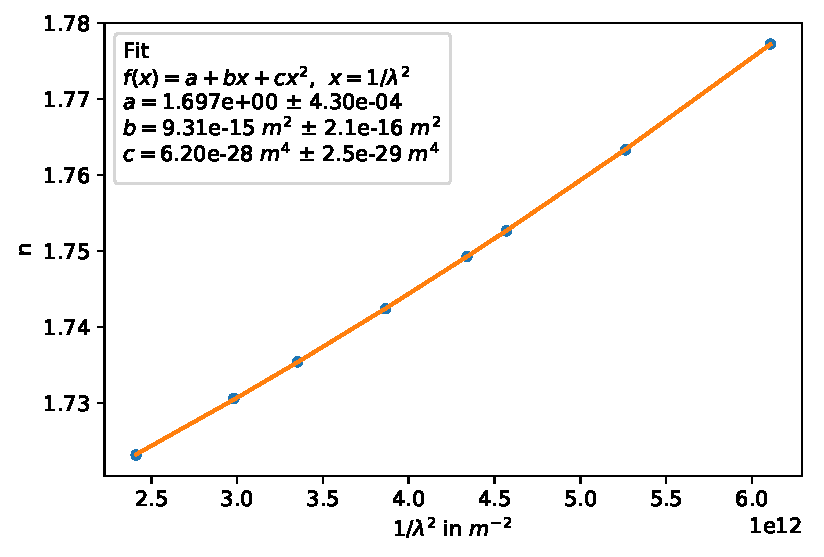
\includegraphics[scale=1]{Python/CdHg_LinReg.pdf}
	\caption{Anpassung der Dispersionskurve mit der Cauchyformel}
	\label{CdHg_LinReg}
\end{figure}

\begin{figure}
	\centering
	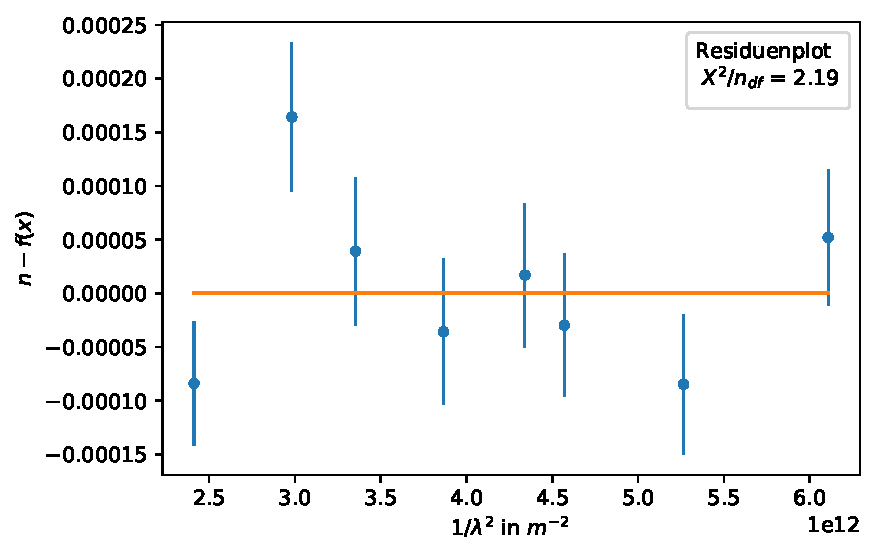
\includegraphics[scale=1]{Python/CdHg_Residuen.pdf}
	\caption{Residuenplot}
	\label{CdHg_Residuenplot}
\end{figure}

\subsection{Untersuchung des Spektrums einer Zinklampe}

\begin{figure}
	\centering
	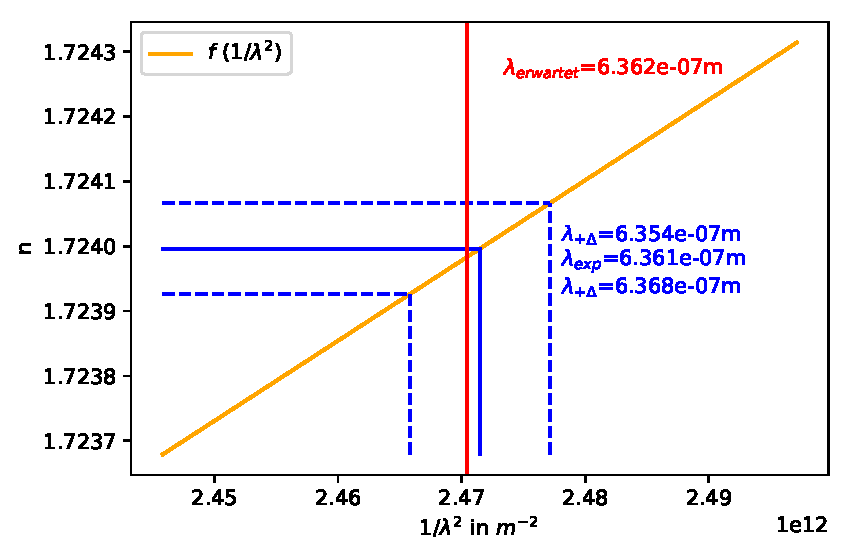
\includegraphics[scale=1]{Python/Zn_0.pdf}
	\caption{Wellenlängenbestimmung des Zinkspektrums: rote Linie. Vergleich mit Literaturwert.}
	\label{Zn_0}
\end{figure}

\begin{figure}
	\centering
	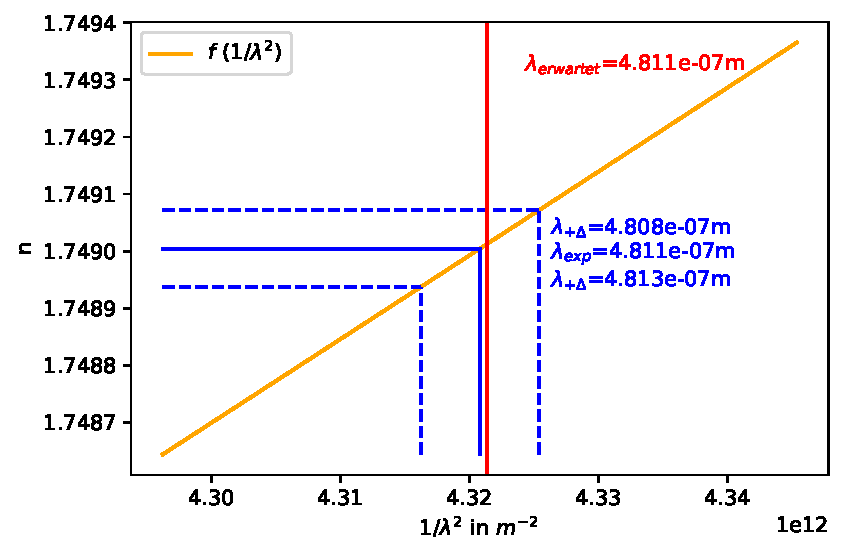
\includegraphics[scale=1]{Python/Zn_1.pdf}
	\caption{Wellenlängenbestimmung des Zinkspektrums: 1. blaue Linie. Vergleich mit Literaturwert.}
	\label{Zn_1}
\end{figure}

\begin{figure}
	\centering
	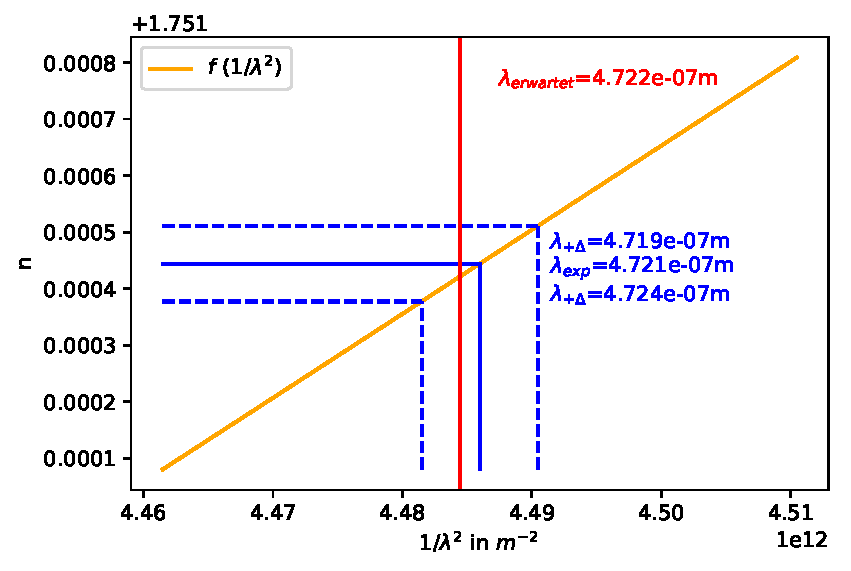
\includegraphics[scale=1]{Python/Zn_2.pdf}
	\caption{Wellenlängenbestimmung des Zinkspektrums: 2. blaue Linie. Vergleich mit Literaturwert.}
	\label{Zn_2}
\end{figure}


\begin{figure}
	\centering
	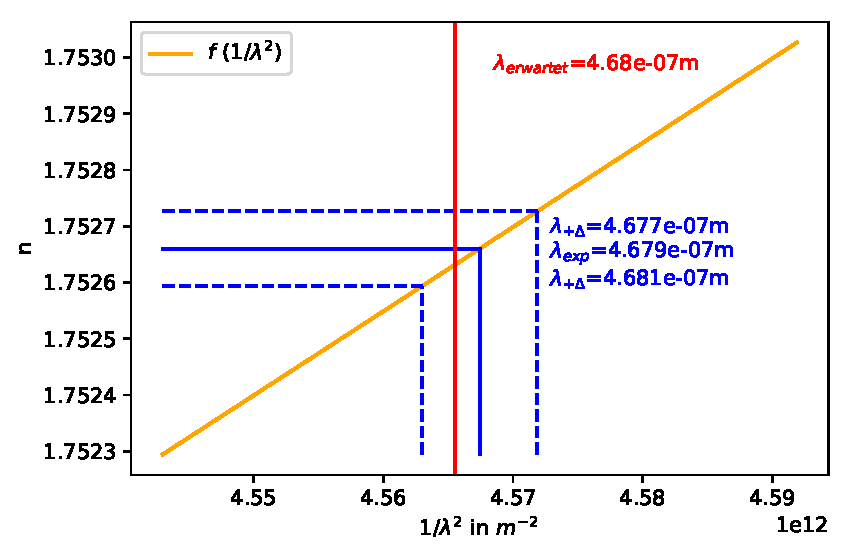
\includegraphics[scale=1]{Python/Zn_3.pdf}
	\caption{Wellenlängenbestimmung des Zinkspektrums: 3. blaue Linie. Vergleich mit Literaturwert.}
	\label{Zn_3}
\end{figure}


\subsection{Auflösungsvermögen}


\end{document}